% ! TeX root = ../../master-thesis.tex

\section{Dynamic Environments}
\label{section:implementation:dynamic-environments}

In support of the test suite, specifically for tests concerning sensors, an
explicit model of dynamic environments has been implemented. In fact, FRASP
provided only an explicit model of static environments, while changes in the
environment were supported with ad-hoc mechanisms, involving direct
modification of the \texttt{SimulationIncarnation} used to define the
specifications.

A basic implementation of a dynamic environment is the
\texttt{EnvironmentWith\-Tags} (Figure \ref{figure:environment-class-diagram}),
which is an \texttt{Environment} where devices can be linked to specific bits
of information, called \textit{tags}. In particular, the methods \texttt{tag}
and \texttt{untag} allow attaching and detaching tags from a set of devices,
while the method \texttt{withTag} can be used to retrieve the time-varying set
of the devices linked to a specific tag.

\begin{figure}[!ht]
  \centering
  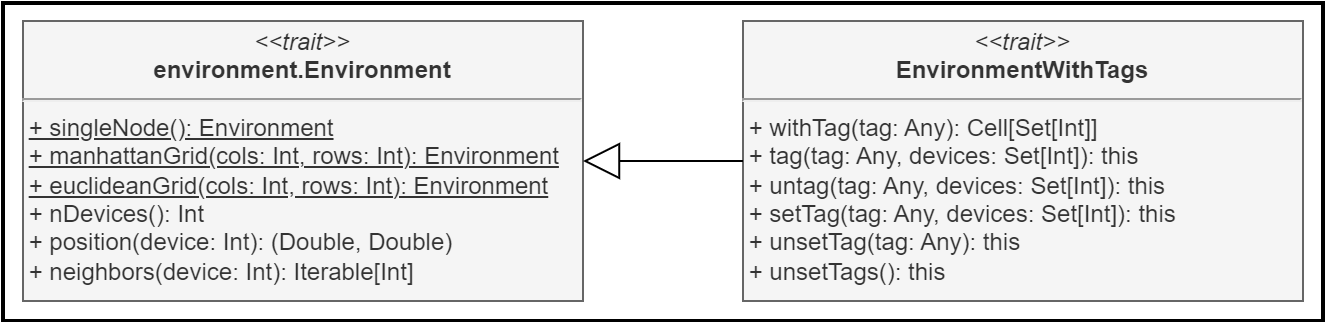
\includegraphics[width=0.8\textwidth]{resources/figures/environment-class-diagram.png}
  \caption[A UML class diagram of the environments types in FRASP]{
    A UML class diagram of the environment types available
    for simulation.
  }
  \label{figure:environment-class-diagram}
\end{figure}

With the introduction of dynamic environments, the
\texttt{SimulationIncarnation} had to be updated to depend on an environment
type, instead of an environment instance (Figure
\ref{figure:simulation-incarnation-class-diagram}). Otherwise, the same
\texttt{SimulationIncarnation} could not be used to define different
specifications, as any program would be executed on the same environment,
already modified by previous programs, possibly causing unpredictable results.

\begin{figure}[!ht]
  \centering
  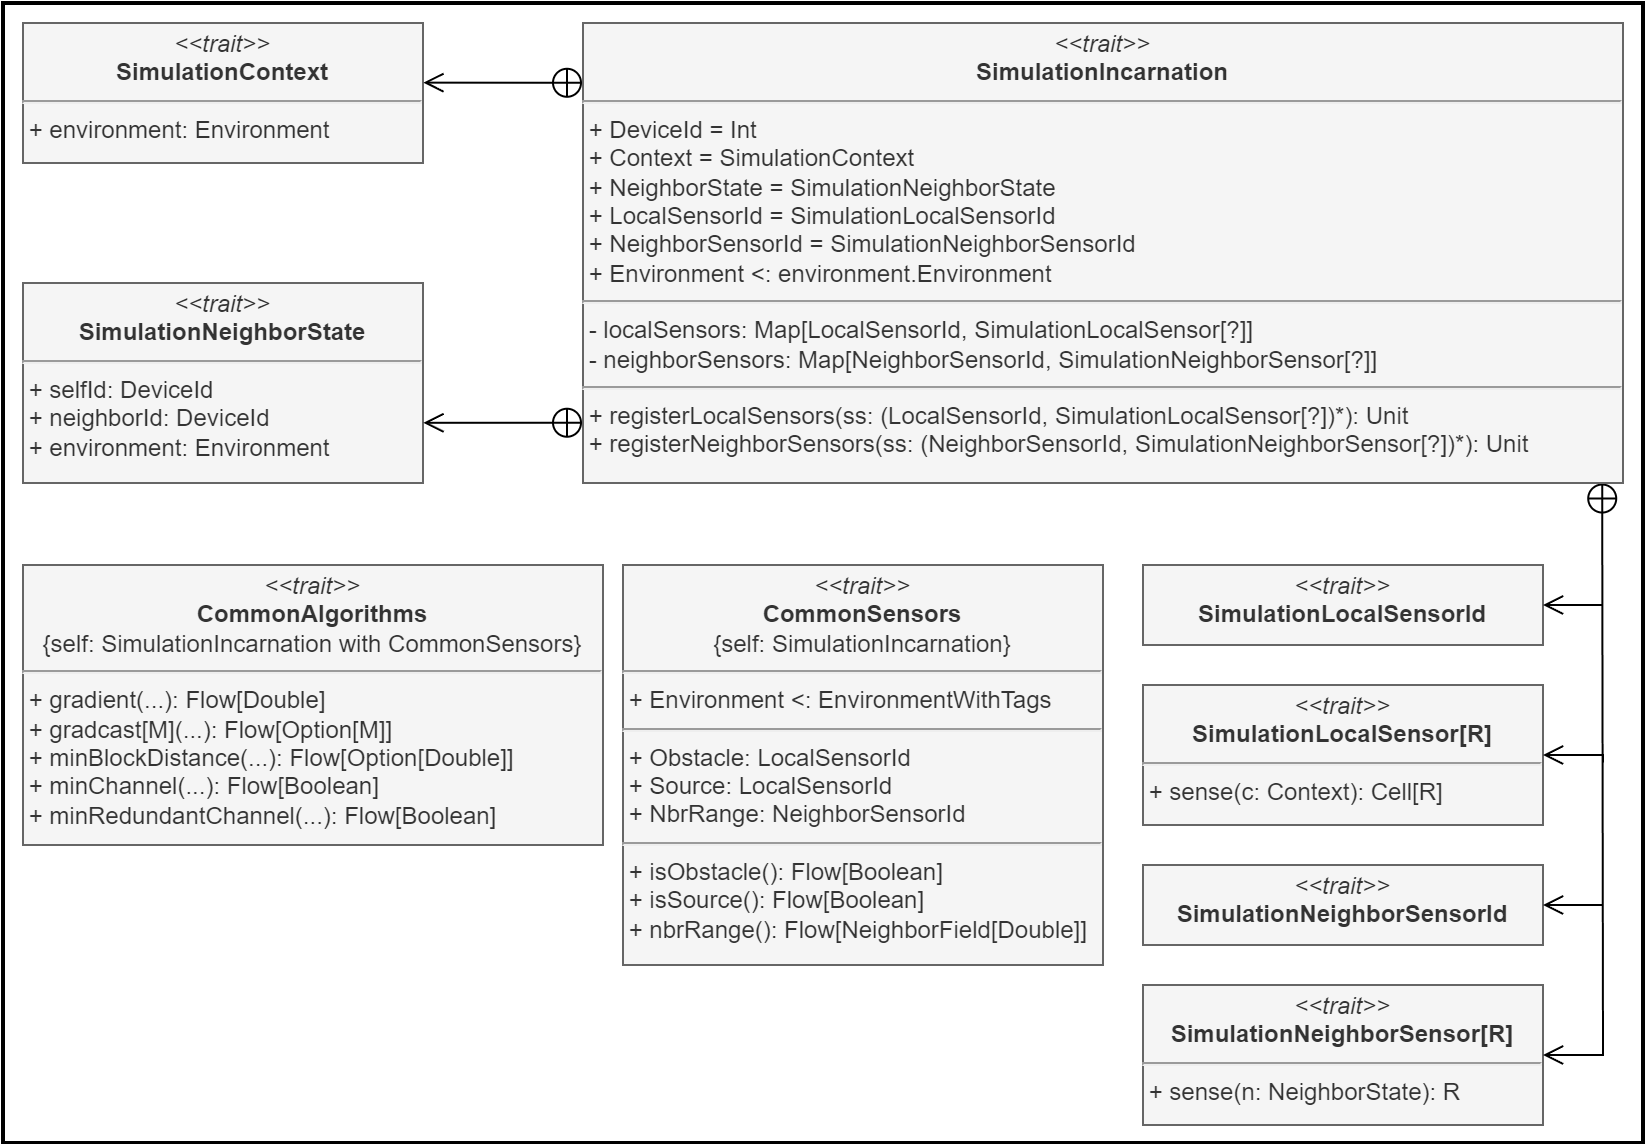
\includegraphics[width=0.85\textwidth]{resources/figures/simulation-incarnation-class-diagram.png}
  \caption[A UML class diagram of the updated simulation incarnation]{
    A UML class diagram of the new \texttt{SimulationIncarnation}.
  }
  \label{figure:simulation-incarnation-class-diagram}
\end{figure}

Additionally, the \texttt{SimulationIncarnation} has been improved to support
the registration of local and neighbor sensors, retrieving localized
information from the environment, instead of relying on information injected
directly into the \texttt{Simu\-lationIncarnation}. In detail, local sensors
are modelled by the trait \texttt{Simula\-tionLocalSensor}, which is a function
producing the readings of a given device in the environment. Local sensors can
be registered to the \texttt{SimulationIncar\-nation} under a specific
identifier, typed \texttt{SimulationLocalSensorId}, by which they can be
referenced using the \texttt{sensor} construct within an aggregate
specification. Similarly, neighbor sensors are implemented by the traits
\texttt{SimulationNeighbor\-Sensor} and \texttt{Simulation\-NeighborSensorId}.

To enhance modularization and isolation of concerns, the implementation of the
sensors has been extracted from the \texttt{SimulationIncarnation} and
delegated to specific traits (Figure \ref{figure:sensor-class-diagram}). In
particular, sensors are modelled by the trait \texttt{Sensor}, which declares
the type of environment where the sensor can be employed, namely
\texttt{SuitableEnviron\-ment}. A \texttt{Sensor} can be either a
\texttt{LocalSensor}, creating the corresponding
\texttt{Simula\-tion\-LocalSensor} for suitable
\texttt{SimulationIncarnation}s, or a \texttt{NeighborSensor}, creating the
corresponding \texttt{SimulationNeighborSensor} for suitable
\texttt{Simulation\-Incarnation}s. A \texttt{SimulationIncarnation} is suitable
for a \texttt{Sensor} if the \texttt{Environ\-ment} of the incarnation is a
\texttt{SuitableEnvironment} for the sensor.

\begin{figure}[!ht]
  \centering
  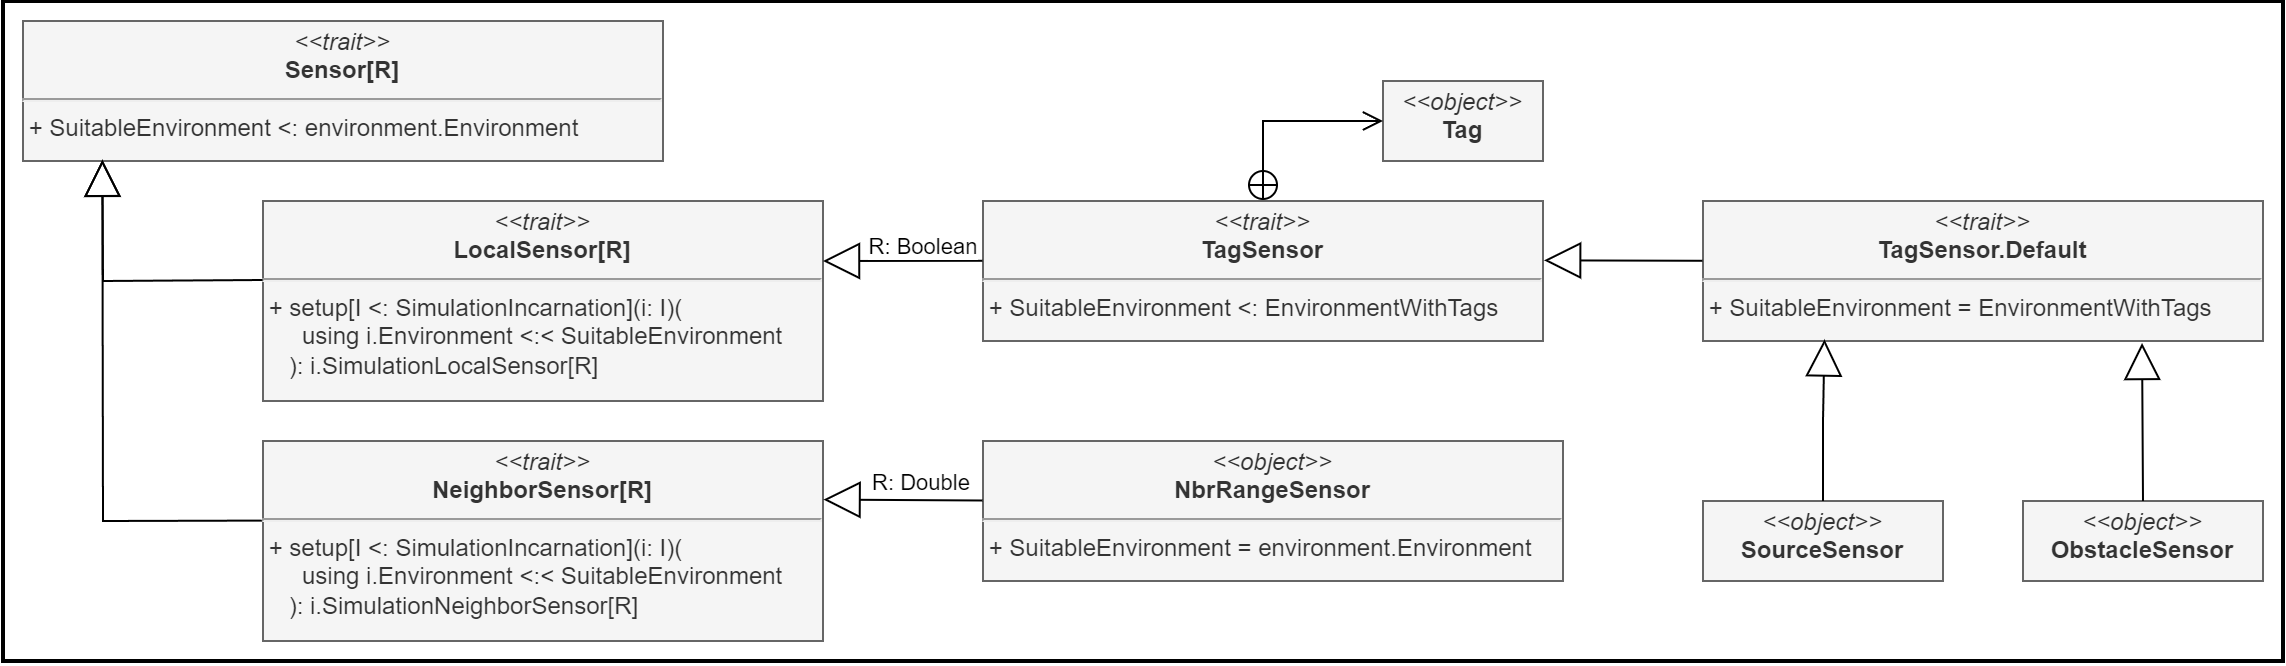
\includegraphics[width=1\textwidth]{resources/figures/sensor-class-diagram.png}
  \caption[A UML class diagram of the sensor types in FRASP]{
    A UML class diagram of the sensor types available for simulation.
  }
  \label{figure:sensor-class-diagram}
\end{figure}

Some built-in sensors have already been implemented, namely \texttt{TagSensor},
which is a \texttt{LocalSensor} detecting if a specific tag is linked to a
device (e.g., if the device is marked as an obstacle or a source), and
\texttt{NbrRangeSensor}, which is a \texttt{NeighborSensor} measuring the
distances from a device and all of its neighbors.

Finally, leveraging these concepts, two mixins for
\texttt{SimulationIncarnation}s have been implemented, namely the
\texttt{CommonSensors} mixin, extending the \ac{DSL} with a set of standard
sensors, and the \texttt{CommonAlgorithms} mixin, extending the \ac{DSL} with a
set of gradient-based algorithms.
